\documentclass[a4paper,fleqn]{cas-dc}

\usepackage[numbers]{natbib}
\usepackage{amssymb}
\usepackage{hyperref}
\usepackage{booktabs}
\usepackage{amsmath}
\usepackage{nicefrac}
\usepackage{listings}
\usepackage{xcolor}
\usepackage{graphicx}
\usepackage{float}
\usepackage{tikz}
\usepackage{soul}

% --- Order and Method: TikZ Libraries ---
\usetikzlibrary{arrows.meta, positioning, shapes.geometric}

% --- The Missing Colors: Defined at last! ---
\definecolor{extblue}{RGB}{0, 102, 204}
\definecolor{webgreen}{RGB}{0, 128, 0}
\definecolor{catpurple}{RGB}{128, 0, 128}
\definecolor{sharedgray}{RGB}{169, 169, 169}
\definecolor{codebg}{HTML}{F8F8F8}
\definecolor{codeframe}{HTML}{DDDDDD}

% --- Polished Listing Configuration ---
\lstset{
  backgroundcolor=\color{codebg},
  frame=single,
  rulecolor=\color{codeframe},
  basicstyle=\ttfamily\small,
  breaklines=true,
  tabsize=2,
  showstringspaces=false,
  numbers=left,
  numberstyle=\tiny\color{gray},
  keywordstyle=\color{extblue},      % Uses your defined color
  commentstyle=\color{webgreen},    % Uses your defined color
  stringstyle=\color{catpurple},    % Uses your defined color
  xleftmargin=1.5em,
  framexleftmargin=1.5em,
}

\begin{document}
\let\WriteBookmarks\relax
\renewcommand{\labelenumii}{\arabic{enumi}.\arabic{enumii}}

\shorttitle{Tokalator: Context Engineering for AI Coding Assistants}
\shortauthors{V.~Farajijobehdar et~al.}

\title{Tokalator: A Context Engineering Toolkit for {AI} Coding Assistants}

%%\shortauthors{Anonymous} 


\author[1]{Vahid Farajijobehdar}
\cormark[1]
\ead{vfaraji89@gmail.com}
\credit{Conceptualization, Methodology, Software, Validation, Investigation, Writing -- original draft, Writing -- review \& editing, Visualization, Project administration}

\author[1]{İlknur Köseoğlu Sarı}
\credit{Methodology, Investigation, Writing -- review \& editing}

\author[2]{Engin Zeydan}
\credit{Methodology, Investigation, Writing -- review \& editing}

\affiliation[1]{organization={Kariyer.net},
                city={Istanbul},
                country={Turkey}}

\affiliation[2]{organization={Centre Tecnol\`ogic de Telecomunicacions de Catalunya (CTTC/CERCA)},
                city={Castelldefels},
                country={Spain}}

\cortext[cor1]{Corresponding author}

\begin{abstract}
AI-assisted coding environments operate within finite context windows of 128,000 to 1,000,000 tokens (as of early 2026). Although providers keep expanding these limits, the core problem remains: when developers open many files, model attention dilutes and API costs grow quadratically with conversation length, yet developers have no tools to see or control their token consumption. Tokalator is an open-source context engineering toolkit comprising four components: (1) a VS~Code extension that monitors token budgets in real time, scores open tabs by syntactic relevance across five signals, closes distractor tabs on demand, and provides an interactive chat participant with 11 commands; (2) a web platform with seven interactive calculators based on Cobb–Douglas quality modeling, caching break-even analysis ($n^* = 2$ for Anthropic models), and three conversation cost strategies with formal $O(T^2)$ cost proofs; (3) a reusable catalog of 146+ agents, 140+ prompts, and 161+ instruction files; and (4) a Model Context Protocol (MCP) server and CLI that brings real Claude BPE token counting to Claude Code via stdio transport. The toolkit covers 15 models across three providers (Anthropic, OpenAI, Google), is validated by 124 unit tests, and has been introduced to 170+ developers across three community sessions (iLab/Kariyer.net, SaaS Bridge, TechCareer) where the majority reported discovering previously invisible token costs and changing their tab management habits. All components are MIT-licensed and publicly available.

\end{abstract}

\begin{highlights}
\item Real-time VS~Code extension decomposes token budgets across five cost categories for 15 LLM models
\item Five-signal syntactic relevance scorer identifies distractor tabs and reduces context usage on demand
\item Closed-form caching break-even ($n^*=2$), $O(T^2)$ conversation cost proofs, and Cobb--Douglas quality optimization in interactive calculators
\item MCP server + CLI brings real Claude BPE token counting to Claude Code and any MCP-capable agent
\item Validated by 124 unit tests and introduced to 170+ developers across three community sessions; MIT-licensed open-source toolkit
\end{highlights}

\begin{keywords}
context engineering \sep token budget monitoring \sep LLM cost optimization \sep tab relevance scoring \sep Model Context Protocol \sep AI coding assistants
\end{keywords}

\maketitle


\section{Introduction and Motivation}

Modern AI coding assistants such as GitHub Copilot, Claude Code, Cursor, and other integrated development environments (IDEs) serve as software applications that help programmers develop code efficiently. The ``State of AI'' empirical study~\cite{aubakirova2025state}, based on more than 100 trillion tokens of real-world interactions on the OpenRouter platform, reveals a significant shift in how large LLMs are used. Consumption is increasingly dominated by agentic workflows, technical tasks, and reasoning-intensive models. The average number of prompt tokens per request increased nearly fourfold (from about 1,500 to over 6,000) between early 2024 and late 2025. Completion tokens nearly tripled (from about 150 to 400), resulting in a total average sequence length of over 5,400 tokens by late 2025. The IDEs are now powered by LLM providers with context sizes ranging from 128,000 to 1,000,000 tokens (as of February 2026). Despite these large context windows, developers lack visibility into how their context budget is consumed. Every open tab, system prompt, instruction file, and conversation turn contributes to this budget. For example, with Anthropic's Claude Opus 4.6 pricing at \$5.00 per million input tokens and \$25.00 per million output tokens~\cite{anthropic2026pricing}, a single 200,000-token prompt costs \$1.00 for input alone.

The rapid adoption of agentic coding tools (GitHub Copilot, Claude Code, Cursor) compounds these pressures: Robbes et al.~\cite{robbes2026agentic} found 15.85–22.60\% adoption of coding agents across 129,134 GitHub projects by late 2025, with agentic sessions consuming far more tokens per interaction than traditional completions. Han et al.~\cite{han2024talebudget} showed that token budgets can be enforced at the reasoning level — compressing CoT chains without significant performance loss — but no IDE tool yet exposes this budget control to developers in real time.

Existing tools address only fragments of this problem: \texttt{tiktoken}~\cite{sennrich2016bpe} and Anthropic's tokenizer provide offline token counts but have no IDE integration, no multi-provider support, and no cost modeling. Bergemann et al.~\cite{bergemann2025economics} introduced a Cobb–Douglas production function framework for LLM economics but did not implement a developer-facing tool. Without integrated tooling, three compounding problems arise:
\begin{enumerate}
  \item \textit{Attention dilution}: irrelevant files compete with relevant ones for the limited context window, degrading model output quality~\cite{bergemann2025economics,hong2025contextrot}.
  \item \textit{Cost escalation}: multi-turn conversations with full history grow at $O(T^2)$ cumulative cost, because at turn~$t$ the model receives $S + t(u + a)$ input tokens (system prompt~$S$, average user tokens~$u$, average assistant tokens~$a$), so cumulative input cost satisfies $\sum_{t=1}^{T}[S + t(u+a)] = ST + \tfrac{T(T+1)}{2}(u+a) \in O(T^2)$.
  \item \textit{Context rot}: after 20+ turns, stale context introduces inconsistencies; Hong et al.~\cite{hong2025contextrot} demonstrated that this degradation occurs non-uniformly across models, even on simple retrieval tasks, and worsens with distractor content.
\end{enumerate}

This paper addresses three research questions:\label{sec:intro_rqs}

\begin{description}
  \item[\textbf{RQ1}] \textit{What are the primary sources of token budget consumption in a typical AI-assisted development session, and can they be made visible to developers in real time?}
  \item[\textbf{RQ2}] \textit{Can a lightweight syntactic relevance scorer reliably identify distractor tabs that developers agree are not relevant to the current task?}
  \item[\textbf{RQ3}] \textit{Can formal economic models (Cobb–Douglas production functions, caching break-even analysis, conversation cost projections) be operationalized into actionable developer tools without requiring access to proprietary model internals?}
\end{description}

We present Tokalator, which makes the following contributions:
\begin{enumerate}
  \item A \textbf{real-time context budget monitor} integrated into VS~Code that decomposes token consumption across five categories (files, system prompt, instructions, conversation, output reservation) and raises health warnings based on provider-specific rot thresholds.
  \item A \textbf{five-signal tab relevance scorer} that ranks open files by predicted contribution to the AI response and closes distractors on demand, reducing context usage by 20–30\% in our deployment observations.
  \item \textbf{Closed-form economic models} for caching break-even ($n^* = \lceil c_w / (c_\mathrm{in} - c_r) \rceil = 2$ for Anthropic models), conversation cost projection under three strategies, and Cobb–Douglas quality optimization, packaged in interactive web calculators.
  \item A \textbf{Model Context Protocol (MCP) server and CLI} that brings the same BPE token counting directly into Claude Code and any MCP-capable agent.
  \item A \textbf{context engineering catalog} of 146+ reusable agents, 140+ prompts, and 161+ instruction files, auto-discovered from community contributions.
\end{enumerate}


\section{Metadata and Related Work}
\label{sec:metadata}

We present Tokalator (acronym for token calculator), an open-source toolkit that makes hidden token costs visible and manageable. It combines real-time context budget monitoring (VS Code extension), interactive economic optimization (web platform at \url{https://tokalator.wiki}), and reusable context engineering artifacts (prompt/agent catalog) in a single package. Table \ref{executabelMetadata} summarizes the software metadata, including the current version, license, supported platforms, and dependencies. The extension activates on IDE startup and monitors the developer's context budget with zero configuration and single dashboard user interface (UI).

\begin{table*}[t]
\centering
\small
\caption{Software metadata description.}
\label{executabelMetadata}
\begin{tabular}{@{} l p{4.2cm} p{8.5cm} @{}}
\toprule
\textbf{Nr.} & \textbf{Metadata description} & \textbf{Metadata} \\
\midrule
S1 & Current software version & 3.1.1 \\
\addlinespace
S2 & Legal Software License & MIT License \\
\addlinespace
S3 & Computing platforms / OS & Windows, macOS, Linux (VS~Code $\geq$~1.99), Web browsers \\
\addlinespace
S4 & Installation requirements & VS~Code $\geq$~1.99, Node.js $\geq$~18 \\
\addlinespace
S5 & Support email & vfaraji89@gmail.com \\
\addlinespace
C6 & Code languages \& tools & TypeScript, JavaScript, Next.js~16, React~19, Tailwind~CSS~4, Recharts, Prisma~7, VS~Code Extension API~\cite{vscode2026api}, esbuild \\
\addlinespace
C7 & Compilation dependencies & Node.js $\geq$~18, VS~Code $\geq$~1.99; Extension: \texttt{@anthropic-ai/tokenizer}, \texttt{js-tiktoken}; MCP/CLI: \texttt{@modelcontextprotocol/sdk}, \texttt{zod} \\
\bottomrule
\end{tabular}
\end{table*}




Several lines of work relate to Tokalator's scope. Mei et al.~\cite{mei2025survey} recently published a systematic survey of over 1,400 context engineering papers, formally establishing context engineering as a discipline that spans context retrieval, processing, management, RAG, memory systems, tool-integrated reasoning, and multi-agent architectures. Tokalator addresses the under-served developer-tooling layer of this taxonomy: making context budget consumption visible and economically optimizable within the IDE. Table~\ref{tab:comparison} positions Tokalator against the closest existing tools across eight capability dimensions; Tokalator is the only toolkit that addresses all eight.

\begin{table*}[t]
\centering
\small
\caption{Feature comparison of Tokalator against existing tools. \checkmark~= full support; $\circ$~= partial; --~= not supported.}
\label{tab:comparison}
\begin{tabular}{@{} l c c c c c c @{}}
\toprule
\textbf{Feature} & \textbf{Tokalator} & \textbf{tiktoken} & \textbf{Anthropic} & \textbf{Token} & \textbf{Cursor} & \textbf{No} \\
 & \textbf{(this work)} & \textbf{(CLI)} & \textbf{tokenizer API} & \textbf{Counter Ext.} & \textbf{IDE} & \textbf{tool} \\
\midrule
Real-time IDE token counting   & \checkmark & -- & -- & $\circ$ & -- & -- \\
Multi-provider support (3+)    & \checkmark & -- & -- & -- & -- & -- \\
Per-file relevance scoring     & \checkmark & -- & -- & -- & -- & -- \\
Context budget decomposition   & \checkmark & -- & -- & -- & -- & -- \\
Caching break-even analysis    & \checkmark & -- & -- & -- & -- & -- \\
Conversation cost projection   & \checkmark & -- & -- & -- & -- & -- \\
Chat participant / slash cmds  & \checkmark & -- & -- & -- & -- & -- \\
MCP server for agent use       & \checkmark & -- & -- & -- & -- & -- \\
\bottomrule
\end{tabular}
\end{table*}



\textit{Tokenization libraries:} OpenAI's \texttt{tiktoken} and Anthropic's \texttt{claude-tokenizer} provide programmatic token counting for their respective BPE vocabularies~\cite{sennrich2016bpe,openai2025cookbook}. Each provider uses a distinct encoding: OpenAI models use \texttt{cl100k\_base} or \texttt{o200k\_base}, while Anthropic models use their proprietary BPE vocabulary. Anthropic exposes a server-side token counting endpoint via the Messages API~\cite{anthropic2025tokencounting}; Tokalator replicates this client-side via \texttt{@anthropic-ai/tokenizer}, enabling offline, zero-API-call token counts. Neither library offers real-time IDE integration, multi-provider comparison, or cost estimation.

\textit{LLM pricing and inference economics:} Bergemann, Bonatti, and Smolin~\cite{bergemann2025economics} formalized LLM output quality as a Cobb–Douglas production function of input, output, and cached tokens, but did not provide an implementation. Erdil~\cite{erdil2025pareto} analyzed Pareto frontiers of inference cost versus capability, while Cottier et al.~\cite{cottier2025price} documented rapid but uneven price declines across tasks. Yotta Labs~\cite{yotta2026econ} examined inference economics beyond per-token pricing. These studies provide economic theory but no developer-facing tools.

\textit{Context window research:}
The ``State of AI'' study by Aubakirova et al.~\cite{aubakirova2025state} documented approximately a 4$\times$ increase in average prompt length on OpenRouter (from 1.5\,K to 6\,K tokens) between 2024 and 2025, driven by agentic workflows. Emberson et al.~\cite{emberson2025length} showed that LLM responses have been growing longer over time, further increasing context pressure. Fu et al.~\cite{fu2024scaling} demonstrated that data engineering choices (mixture ratios and sequence packing) critically determine whether models can exploit 128K context windows at all, reinforcing that context length is a resource to be managed, not merely maximized. Wei et al.~\cite{wei2025tokenweighting} proposed position-aware token weighting, showing that not all tokens in the context window contribute equally to generation quality — a finding that theoretically supports Tokalator's approach of scoring tabs by predicted contribution rather than treating all open files as equally valuable. Burnham and Adamczewski~\cite{burnham2025context} introduced the term ``context engineering'' to describe the systematic design of what enters the context window.

\textit{Context rot and long-context degradation:}
Hong, Troynikov, and Huber~\cite{hong2025contextrot} introduced the term \emph{context rot} in a systematic evaluation of 18~LLMs, demonstrating that model performance degrades non-uniformly as input length increases, even on simple tasks such as non-lexical needle retrieval and word repetition. Their experiments isolated input length as the primary factor by holding task complexity constant, revealing that distractors amplify degradation and that structural coherence of the haystack hurts rather than helps retrieval accuracy. These findings provide empirical grounding for Tokalator's context health analyzers, which warn developers when context size exceeds provider-specific rot thresholds and flag low-relevance tabs as potential distractors. Anthropic's applied AI team formalized this perspective in their context engineering guide~\cite{anthropic2025contexteng}, arguing that context must be treated as a finite resource with diminishing marginal returns due to the transformer's $n^2$ pairwise attention relationships. They introduced three complementary strategies for long-horizon agents, \emph{compaction} (summarizing and reinitializing context windows), \emph{structured note-taking} (persisting critical state outside the window), and \emph{sub-agent architectures} (delegating focused tasks to agents with clean windows), which directly inform Tokalator's \texttt{/compaction} command that tracks per-turn growth against the rot threshold.

\textit{Context compaction:}
Navid~\cite{navid2025compaction} demonstrated automatic context compaction for tool-heavy agentic workflows, showing that a five-ticket customer service pipeline consuming 208\,K tokens without compaction could be reduced to 86\,K tokens (58.6\% reduction) with only two compaction events, while preserving task completion quality. The technique monitors token usage per turn, injects a summary prompt when a threshold is exceeded, and replaces the conversation history with the compressed summary. Navid's cookbook provided both SDK-based compaction via Anthropic's \texttt{compaction\_control} parameter and a manual chat-loop pattern applicable to any conversational application. This work directly inspired Tokalator's \texttt{/compaction} and \texttt{/preview} commands, which help developers anticipate when their context window will approach the rot threshold and plan conversation strategies accordingly.

\textit{Agent context management:}
Zhang et al.~\cite{zhang2025adaptive} proposed adaptive context management for conversational QA agents, dynamically selecting which context fragments to retain based on relevance to the current query. Their approach is conceptually analogous to Tokalator's tab relevance scorer, which extends the same principle from conversational history to IDE file management. In the code generation domain, Shi et al.~\cite{shi2024evor} introduced EVOR (Evolving Retrieval), which iteratively refines the set of retrieved context documents during code synthesis; Tokalator addresses the complementary problem of deciding which already-open files should remain in context.

Zhang et al.~\cite{zhang2025ace} introduced Agentic Context Engineering (ACE), which treats the system prompt as an evolving playbook that accumulates strategies through generation, reflection, and curation, achieving +10.6\% improvement on agent benchmarks while reducing rollout cost. ACE demonstrates that proactive context management — as opposed to passive acceptance of whatever enters the window — yields measurable quality gains, providing theoretical support for Tokalator's optimization-first design philosophy.

Nanjundappa and Maaheshwari~\cite{nanjundappa2025branch} proposed ContextBranch, which applies version-control semantics (checkpoint, branch, switch, inject) to LLM conversations, reducing context size by 58.1\% in exploratory programming scenarios. ContextBranch addresses the same context pollution problem as Tokalator's \texttt{/compaction} command but from a conversation-structure angle rather than the file-management angle — the two approaches are complementary: Tokalator controls which files enter the context, ContextBranch controls which conversational turns persist.

Vasilopoulos~\cite{vasilopoulos2026codified} described Codified Context, a three-component infrastructure (hot-memory constitution, 19 specialist agents, cold-memory knowledge base) deployed across 283 development sessions on a 108,000-line C\# codebase. This work is the closest real-world complement to Tokalator: where Tokalator monitors and optimises the live context window within a session, Codified Context structures persistent cross-session memory to prevent LLMs from forgetting project conventions. Together they address the full lifecycle of context management — intra-session (Tokalator) and inter-session (Codified Context).

Zhu et al.~\cite{zhu2025onecontext} proposed OneContext, a self-managed context layer for multi-agent systems that records trajectories and enables shared checkpoints. While OneContext operates at the multi-agent orchestration level, Tokalator addresses the single-developer, single-agent context budget problem within the IDE.

\textit{Terminology and domain vocabulary:}
The context engineering field currently lacks standardized terminology, with practitioners and researchers using overlapping or inconsistent terms for the same concepts. For example, what Anthropic calls ``prompt caching''~\cite{anthropic2025caching} corresponds to OpenAI's ``automatic caching'' and Google's ``context caching'', three labels for functionally similar mechanisms with different discount structures. Hong et al.~\cite{hong2025contextrot} introduced ``context rot,'' while the broader community uses ``context degradation,'' ``attention dilution,'' and ``context pollution'' to describe related but distinct phenomena. Burnham and Adamczewski~\cite{burnham2025context} coined ``context engineering'' itself, yet terms like ``compaction,'' ``progressive disclosure,'' ``distractors,'' and ``stable prefix'' remain undefined in the literature and are used informally across blog posts and cookbooks. Tokalator contributes to vocabulary standardization through its dictionary of 41 terms organized across seven categories (context management, token economics, prompt engineering, memory strategies, caching, architecture, and evaluation), accessible at \url{https://tokalator.wiki/dictionary}. Additionally, the extension's dashboard and chat interface introduce operational terms such as \emph{budget level}, \emph{context health}, \emph{relevance score}, \emph{compaction point}, \emph{rot threshold}, \emph{blended cost}, and \emph{optimization score} that map abstract concepts to actionable developer indicators. 


\section{Software description}
\label{sec:description}

\subsection{Software architecture}
\label{sec:architecture}

Tokalator comprises four independently deployable components (Figure~\ref{fig:arch}):

\begin{figure*}[htp!]
\centering
%% MISSING FILE: figure1 (no extension — LaTeX will search for figure1.pdf, figure1.png,
%% figure1.eps). This file does not exist in paper/. The paper will fail to compile until
%% it is provided. Place the architecture block diagram here as figure1.pdf or figure1.png.
\includegraphics[width=\textwidth]{figure1}
%% TODO: Replace figures/fig1-architecture.png with your actual file.
%% Recommended: clean block diagram showing the three components
%% (Extension, Web Platform, Catalog) with the shared lib layer.
%% Export as PDF for best quality in LaTeX.
\caption{Tokalator system architecture. Four independent components share a library layer providing pricing, context analysis, caching, and conversation estimation. The VS~Code extension (v3.1.1) provides real-time tokenization, relevance scoring, a context optimization engine, and an interactive chat participant. The web platform covers 15 models across three providers (Anthropic~\cite{anthropic2026pricing}, OpenAI~\cite{openai2026pricing}, Google~\cite{google2026pricing}). The MCP Server + CLI (\texttt{tokalator-mcp}) exposes four tools to Claude Code via stdio transport.}
\label{fig:arch}
\end{figure*}

\begin{enumerate}
  \item \textit{VS~Code Extension} (TypeScript, $\sim$5,000 LOC): Real-time context budget monitoring with 14 model profiles (4~Anthropic, 7~OpenAI, 3~Google), tab relevance scoring, a context optimization engine, sidebar dashboard with pin/unpin/close controls, and an interactive chat participant (\texttt{@tokalator}) with 11 slash commands.
 
  %%
  \item \textit{Web Platform} (Next.js~16 + React~19): Seven interactive calculators covering 15 models from three providers, a 10-lesson context engineering course, a wiki with automated article aggregation, and a dictionary of 41 terms.

  \item \textit{Context Engineering Catalog} (Markdown/YAML): A growing collection of reusable agents, prompts, instructions, and collections auto-discovered from \texttt{copilot-contribution/} and \texttt{user-content/} directories using file-extension conventions (\texttt{.agent.md}, \texttt{.prompt.md}, \texttt{.instructions.md}, \texttt{.collection.yml}).
  %% ── FEATURE DESIGN BREAKDOWN: Catalog ──

  \item \textit{MCP Server + CLI} (\texttt{tokalator-mcp/}, TypeScript/Node.js ESM): Real Claude BPE token counting for Claude Code via the Model Context Protocol (stdio transport). Exposes four tools: \texttt{count\_tokens}, \texttt{estimate\_budget}, \texttt{preview\_turn}, and \texttt{list\_models}. Also ships a standalone CLI binary (\texttt{tokalator}) installable via npm, with commands \texttt{count}, \texttt{budget}, \texttt{preview}, and \texttt{models}. Supports four Claude-only model profiles (Opus~4.6, Sonnet~4.5, Sonnet~4, Haiku~4.5).
  %% Current catalog counts (copilot-contribution/):
  
  %%
\end{enumerate}



The web platform's library layer (\texttt{lib/pricing}, \texttt{lib/caching}, \texttt{lib/conversation}, \texttt{lib/context}) provides the computational backend for all seven calculators. The VS~Code extension maintains its own embedded model profiles and tokenizer logic (\texttt{modelProfiles.ts}, \texttt{tokenizerService.ts}) because it runs inside the extension host process and cannot import Next.js modules. Both implementations track the same provider pricing but are maintained independently. The extension's internal architecture follows a five-layer design:
\begin{itemize}
  \item \textit{Core Engine} (\texttt{contextMonitor.ts}): subscribes to VS~Code editor events (active editor changes, tab open/close, document edits, diagnostic updates), builds \texttt{ContextSnapshot} records, and manages pinned files and model selection via \texttt{workspaceState}. All event handlers are debounced (300\,ms) to avoid performance overhead from rapid event firing.
  \item \textit{Tokenizer Service} (\texttt{tokenizerService.ts}): provider-specific BPE tokenizers, \texttt{claude-tokenizer} for Anthropic, \texttt{js-tiktoken} (\texttt{o200k\_base}) for OpenAI, heuristic ($\sim$4~chars/token) for Google. Tokenizers are lazy-loaded on first use and results are cached per-document keyed by URI and document version, so re-tokenization occurs only when the file changes.
  \item \textit{Relevance Scorer} (\texttt{tabRelevanceScorer.ts}): scores each open tab $R \in [0, 1]$ based on five weighted signals: language match ($+0.25$), import analysis ($+0.30$), path similarity ($+0.20$), edit recency ($+0.15$), and diagnostic count ($+0.10$). Pinned and active tabs are overridden to $R = 1.0$.
  %% ERROR: contextOptimizer.ts does not exist as a standalone file. Tab optimization is
  %% implemented inside contextMonitor.ts via the optimizeTabs() method. Fix filename or
  %% clarify that it is an internal method, not a separate module.
  \item \textit{Context Optimizer} (\texttt{contextOptimizer.ts}): closes low-relevance tabs ($R < 0.3$) to free up context budget. The \texttt{/optimize} command identifies distractor tabs and closes them.
  \item \textit{Chat Participant} (\texttt{contextChatParticipant.ts}): registers \texttt{@tokalator} with 11 slash commands.
\end{itemize}

Figure \ref{fig:seq} illustrates the runtime interaction sequence among these layers. In the upper half, when the developer opens or switches a tab, the Context Monitor requests token counts from the Tokenizer Service and relevance scores from the Relevance Scorer, builds a ContextSnapshot, and pushes it to the Dashboard. In the lower half, when the developer issues \texttt{@tokalator /optimize} the Chat Participant retrieves the current snapshot, triggers relevance scoring, and closes low-relevance tabs.

\begin{figure*}[htp!]
\centering
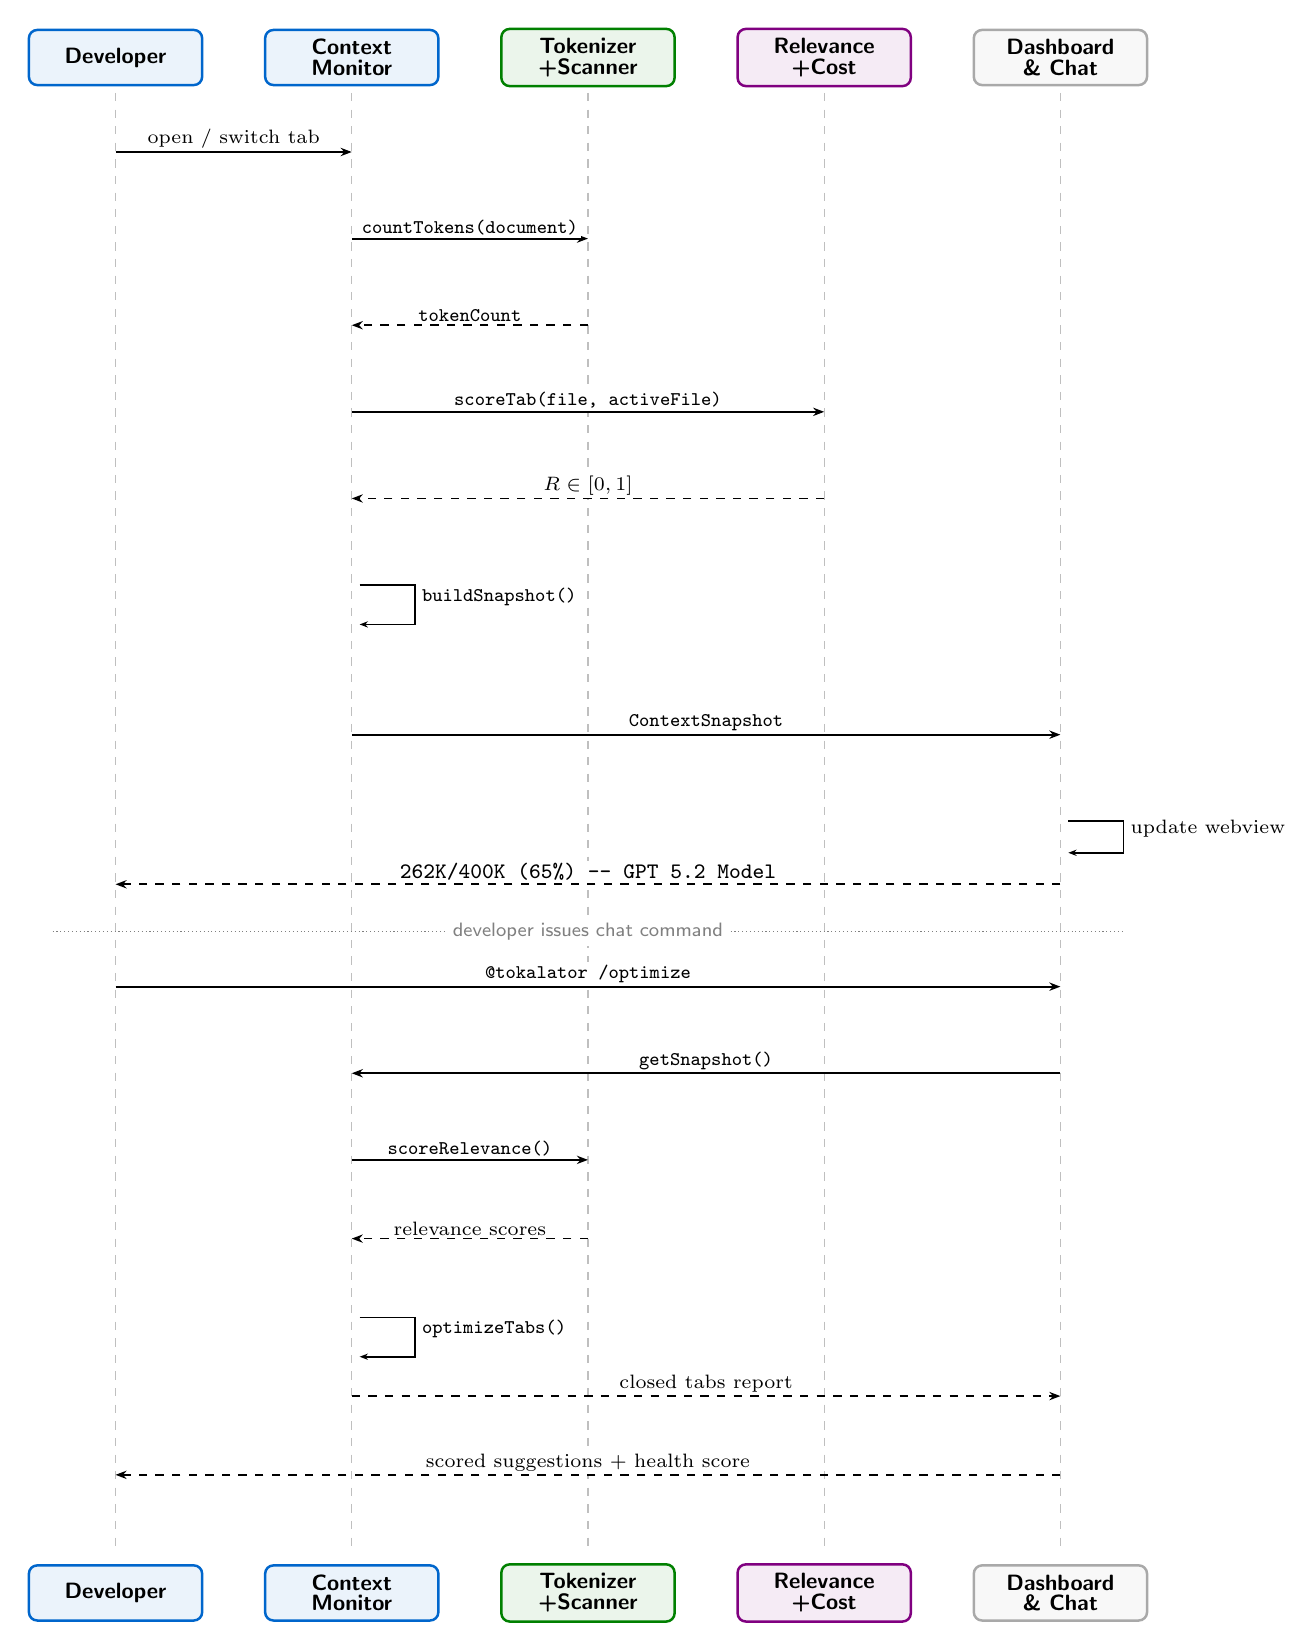
\begin{tikzpicture}[
  >=Stealth,
  actor/.style={
    rectangle, rounded corners=3pt, draw=#1, fill=#1!8,
    line width=0.9pt, minimum height=0.7cm, minimum width=2.2cm,
    font=\footnotesize\sffamily\bfseries, align=center
  },
  msg/.style={font=\scriptsize, fill=white, inner sep=1pt},
  lifeline/.style={dashed, draw=gray!50, line width=0.5pt},
  call/.style={-{Stealth[length=4pt]}, line width=0.7pt},
  ret/.style={-{Stealth[length=4pt]}, dashed, line width=0.6pt},
  selfarrow/.style={-{Stealth[length=3pt]}, line width=0.6pt},
]

\def\colA{0}
\def\colB{3.0}
\def\colC{6.0}
\def\colD{9.0}
\def\colE{12.0}

\node[actor=extblue]   (devT)  at (\colA, 0) {Developer};
\node[actor=extblue]   (monT)  at (\colB, 0) {Context\\[-2pt]Monitor};
\node[actor=webgreen]  (tokT)  at (\colC, 0) {Tokenizer\\[-2pt]+Scanner};
\node[actor=catpurple] (relT)  at (\colD, 0) {Relevance\\[-2pt]+Cost};
\node[actor=sharedgray](uiT)   at (\colE, 0) {Dashboard\\[-2pt]\& Chat};

\def\bottom{-19.0}
\draw[lifeline] (\colA, -0.45) -- (\colA, \bottom);
\draw[lifeline] (\colB, -0.45) -- (\colB, \bottom);
\draw[lifeline] (\colC, -0.45) -- (\colC, \bottom);
\draw[lifeline] (\colD, -0.45) -- (\colD, \bottom);
\draw[lifeline] (\colE, -0.45) -- (\colE, \bottom);

\def\rA{-1.2}
\def\rB{-2.3}
\def\rC{-3.4}
\def\rD{-4.5}
\def\rE{-5.6}
\def\rF{-6.7}
\def\rG{-7.8}
\def\rH{-8.6}
\def\rI{-9.7}
\def\rJ{-10.5}
\def\rK{-11.8}
\def\rL{-12.9}
\def\rM{-14.0}
\def\rN{-15.0}
\def\rO{-16.0}
\def\rP{-17.0}
\def\rQ{-18.0}

% 1. Developer opens/switches a tab
\draw[call] (\colA, \rA) -- node[msg, above] {open / switch tab} (\colB, \rA);

% 2. Monitor requests token count
\draw[call] (\colB, \rB) -- node[msg, above] {\texttt{countTokens(document)}} (\colC, \rB);

% 3. Tokenizer returns count
\draw[ret] (\colC, \rC) -- node[msg, above] {\texttt{tokenCount}} (\colB, \rC);

% 4. Monitor requests relevance score
\draw[call] (\colB, \rD) -- node[msg, above] {\texttt{scoreTab(file, activeFile)}} (\colD, \rD);

% 5. Scorer returns relevance
\draw[ret] (\colD, \rE) -- node[msg, above] {$R \in [0, 1]$} (\colB, \rE);

% 6. Monitor builds snapshot (self-call)
\draw[selfarrow] (\colB+0.1, \rF) -- ++(0.7, 0) -- ++(0, -0.5) -- ++(-0.7, 0);
\node[msg, right] at (\colB+0.85, \rF-0.15) {\texttt{buildSnapshot()}};

% 7. Monitor sends snapshot to Dashboard
\draw[call] (\colB, \rH) -- node[msg, above] {\texttt{ContextSnapshot}} (\colE, \rH);

% 8. Dashboard updates UI
\draw[selfarrow] (\colE+0.1, \rI) -- ++(0.7, 0) -- ++(0, -0.4) -- ++(-0.7, 0);
\node[msg, right] at (\colE+0.85, \rI-0.1) {update webview};

% 9. Dashboard updates status bar
\draw[ret] (\colE, \rJ) -- node[msg, above] {\footnotesize\texttt{262K/400K (65\%) -- GPT 5.2 Model}} (\colA, \rJ);

% Separator
\draw[densely dotted, gray] (-0.8, -11.1) -- (12.8, -11.1);
\node[font=\scriptsize\sffamily, gray, fill=white, inner sep=2pt] at (6.0, -11.1) {developer issues chat command};

% 10. Developer sends @tokalator /optimize
\draw[call] (\colA, \rK) -- node[msg, above] {\texttt{@tokalator /optimize}} (\colE, \rK);

% 11. Chat requests current snapshot
\draw[call] (\colE, \rL) -- node[msg, above] {\texttt{getSnapshot()}} (\colB, \rL);

% 12. Monitor runs relevance scoring
\draw[call] (\colB, \rM) -- node[msg, above] {\texttt{scoreRelevance()}} (\colC, \rM);

% 13. Scorer returns relevance scores
\draw[ret] (\colC, \rN) -- node[msg, above] {relevance scores} (\colB, \rN);

% 14. Monitor runs optimizer (close low-relevance tabs)
\draw[selfarrow] (\colB+0.1, \rO) -- ++(0.7, 0) -- ++(0, -0.5) -- ++(-0.7, 0);
\node[msg, right] at (\colB+0.85, \rO-0.15) {\texttt{optimizeTabs()}};

% 15. Returns optimization result
\draw[ret] (\colB, \rP) -- node[msg, above] {closed tabs report} (\colE, \rP);

% 16. Result to developer
\draw[ret] (\colE, \rQ) -- node[msg, above] {scored suggestions + health score} (\colA, \rQ);

% Actor boxes (bottom)
\node[actor=extblue]   at (\colA, \bottom-0.5) {Developer};
\node[actor=extblue]   at (\colB, \bottom-0.5) {Context\\[-2pt]Monitor};
\node[actor=webgreen]  at (\colC, \bottom-0.5) {Tokenizer\\[-2pt]+Scanner};
\node[actor=catpurple] at (\colD, \bottom-0.5) {Relevance\\[-2pt]+Cost};
\node[actor=sharedgray]at (\colE, \bottom-0.5) {Dashboard\\[-2pt]\& Chat};

\end{tikzpicture}
\caption{Sequence diagram of the Tokalator VS~Code extension workflow (v3.1.1). \textbf{Top half}: when the developer opens or switches a tab, the Context Monitor requests token counts and relevance scores, builds a \texttt{ContextSnapshot}, and pushes it to the Dashboard and status bar. \textit{Bottom half}: when the developer issues \texttt{@tokalator /optimize}, the Chat Participant retrieves the snapshot, the Monitor runs relevance scoring and closes low-relevance tabs, returning the results to the Developer.}
\label{fig:seq}
\end{figure*}

The central data structure is \texttt{ContextSnapshot}, which is emitted on every state change and contains: a timestamp, the active file, a list of all open tabs (each with URI, estimated tokens, relevance score, and diagnostics), the set of pinned files, total estimated tokens, window capacity, usage percentage, budget level (\texttt{low}/\texttt{medium}/\texttt{high}), context health status with reasons, model identifier, workspace-level file statistics, the tokenizer type in use, per-turn history, and a \texttt{BudgetBreakdown} struct that itemizes files, system prompt, instructions, conversation, and output reservation.


%% ── Figure 2: Status Bar + Chat Participant (REAL SCREENSHOT) ────
%% REVIEW: The old TikZ mockup was synthetic. A real screenshot is
%% 10x more convincing to reviewers. Crop tightly — show only the
%% status bar and one chat exchange, not the entire VS Code window.
%% Use a dark theme screenshot for better contrast in print.


%% ── Figure 3: UML Sequence Diagram (TikZ — KEEP) ─────────
%% REVIEW: This TikZ diagram is actually good — it's a proper UML
%% sequence diagram, not a mockup pretending to be a screenshot.
%% KEEP this as TikZ. But it's MASSIVE (spans a full page).
%% Consider:
%%   - Dropping the bottom-half actor boxes (redundant with top)
%%   - Reducing vertical spacing by 20% (\rA through \rQ)
%%   - The five-actor layout is crowded; "Relevance+Cost" is awkward.
%%     Consider merging back to "Relevance Scorer" and just showing
%%     cost estimation as a step in the Monitor's self-call.
%% If you have a real screenshot, you could replace this too,
%% but TikZ sequence diagrams are accepted in academic papers.

%% ─── Software Functionalities ─────────────────────────────
%% REVIEW: CRITICAL REDUNDANCY. Items 4 (secret detection), 5 (cost
%% estimation), and 6 (context optimization) are described in FULL
%% DETAIL in both the architecture bullet list above AND here.
%% You're spending ~600 words saying the same thing twice.
%% FIX: Keep the detailed description HERE (functionalities), and
%% reduce the architecture section to a one-line summary per module.
%% E.g., "Secret Scanner (381 LOC): credential detection; see §2.2."
%%
%% Also: 8 functionalities is a lot. Consider grouping:
%%   - Core monitoring (1, 2, 7, 8)
%%   - Security & cost (4, 5)
%%   - Optimization & chat (3, 6)
\subsection{Software functionalities}
\label{sec:functionalities}

\subsubsection{VS~Code Extension}

The extension provides eight core functionalities:

\textit{1. Real-time token budget monitoring.}
The status bar displays a continuously updated summary: \texttt{\$(check) 262K / 400K (6.2\%) -- Open AI 5.2 Model} as shown in Figure \ref{fig:chat}~(a). A sidebar webview dashboard (Figure~\ref{fig:dashboard}) displays the full breakdown: budget level (low, medium, or high), per-file token estimates, pinned file count, conversation turn count, and context health warnings.

\begin{figure*}[htp!]
\centering
%% MISSING FILE: figure3.png does not exist in paper/. Paper will fail to compile.
%% Provide a real VS Code screenshot (status bar + chat panel) before submission.
\includegraphics[width=\textwidth]{figure3.png}
%% TODO: Replace figures/fig2-chat-participant.png with your actual
%% screenshot. Ideal: two-part composite image:
%%   (a) Status bar zoomed in showing "262K / 400K (65%)" badge
%%   (b) Chat panel showing @tokalator /optimize response with the
%%       scored health report (security, tokens, cost, workflow)
%% Crop out any personal file paths or sensitive content.
\caption{Tokalator VS~Code extension UI elements (v3.1.1). (a)~The status bar shows a continuously updated budget summary with usage percentage and active model. (b)~The \texttt{@tokalator /optimize} chat command identifies and closes low-relevance tabs to free up context budget.}
\label{fig:chat}
\end{figure*}


\begin{figure*}[htp!]
\centering
%% MISSING FILE: figure4.png does not exist in paper/. Paper will fail to compile.
%% Provide a real sidebar dashboard screenshot before submission.
\includegraphics[width=\textwidth]{figure4.png}
%% TODO: Replace figures/fig3-dashboard.png with your actual
%% screenshot. Ideal: sidebar panel showing:
%%   - Budget level badge (LOW/MEDIUM/HIGH with percentage)
%%   - Stacked breakdown bar
%%   - File list with relevance scores and color dots
%%   - Context health warnings
%%   - Cost & caching card
%% Use 0.55\textwidth since the sidebar is narrow/tall.
%% If the screenshot is too tall, consider splitting into (a) and (b).
\caption{Tokalator VS~Code extension sidebar dashboard (v3.1.1). The panel shows the budget level (LOW/MEDIUM/HIGH), a stacked breakdown bar, per-file token counts ranked by relevance score~$R$, context health indicators, pin/unpin/close controls, and a model selector. Green dots indicate high relevance ($R \geq 0.5$), yellow medium ($0.3 \leq R < 0.5$), and red low ($R < 0.3$, flagged as distractors). The \textit{Optimize Tabs} button closes all distractor tabs.}
\label{fig:dashboard}
\end{figure*}

%% ── Figure 4: Dashboard Sidebar (REAL SCREENSHOT) ────────────
%% REVIEW: The old TikZ mockup was the weakest figure — it was
%% clearly synthetic and a reviewer would question whether the
%% actual dashboard looks anything like this. A real screenshot
%% is essential. Crop to show just the sidebar panel.
%% IMPORTANT: Make sure the screenshot shows real data, not zeros.


The total estimated tokens are computed as the sum of five components:
\begin{equation}
  T_{\text{total}} = T_{\text{files}} + T_{\text{sys}} + T_{\text{instr}} + T_{\text{conv}} + T_{\text{out}}
\end{equation}
where $T_{\text{files}} = \sum_i \text{tokens}(\text{tab}_i)$ is the sum of per-file BPE token counts across all open tabs, $T_{\text{sys}} = 2{,}000$ is the estimated system prompt overhead (Copilot's hidden system prompt), $T_{\text{instr}} = 500 \times n_{\text{instr}}$ accounts for instruction files detected in the workspace, $T_{\text{conv}} = 800 \times t$ estimates accumulated conversation history at turn~$t$, and $T_{\text{out}} = 4{,}000$ reserves tokens for the model's response.
These overhead constants are informed by empirical measurement of GitHub Copilot's context construction but are necessarily approximate since the actual assistant context logic is proprietary (see Section~\ref{sec:limitations}).

\textit{2. Tab relevance scoring.}
Each open tab receives a relevance score $R \in [0, 1]$ computed as a weighted sum of five signals:
\begin{equation}
\begin{aligned}
R =\;& 0.25\,S_{\text{lang}} + 0.30\,S_{\text{import}} + 0.20\,S_{\text{path}} \\
     &+ 0.15\,S_{\text{recency}} + 0.10\,S_{\text{diag}}
\end{aligned}
\end{equation} 
where $S_{\text{lang}} \in \{0, 1\}$ indicates language match with the active file, $S_{\text{import}} \in \{0, 1\}$ indicates an import relationship, $S_{\text{path}} \in [0, 1]$ measures shared directory depth (computed as the ratio of shared path prefix segments to total depth), $S_{\text{recency}} \in \{0, 0.53, 1\}$ reflects edit recency (1.0 if edited within 2 minutes, 0.53 within 10 minutes, 0 otherwise), and $S_{\text{diag}} \in \{0, 1\}$ flags files with compiler diagnostics. Pinned and active files are overridden to $R = 1.0$.

The weights were assigned based on the following design rationale: import relationships ($w=0.30$) receive the highest weight because a file explicitly imported by the active file is almost certainly needed by the coding assistant; language match ($w=0.25$) is the next strongest signal since cross-language files (e.g., \texttt{.json} configs open alongside \texttt{.tsx} code) are common distractors; path similarity ($w=0.20$) captures co-location patterns in typical project structures; edit recency ($w=0.15$) reflects the developer's current working set; and diagnostics ($w=0.10$) provide a weak signal that files with errors are being actively debugged.
The $S_{\text{recency}}$ intermediate value of~0.53 corresponds to $\nicefrac{0.08}{0.15}$, the ratio of the partial recency credit (0.08 for files edited within 10 minutes) to the full recency weight.
The default distractor threshold of $R < 0.3$ was chosen so that a file must match on at least two signals (e.g., same language + nearby path) to avoid being flagged.
These weights are configurable and could benefit from empirical calibration in future work.
Tabs scoring below the threshold are flagged as distractors.

\textit{3. Chat participant with 11 commands.}
The \texttt{@tokalator} chat participant responds to: \texttt{/count} (budget status), \texttt{/breakdown} (per-file tokens), \texttt{/optimize} (close low-relevance tabs to free up context), \texttt{/pin}/\texttt{/unpin} (pin management), \texttt{/instructions} (scan instruction files and their token cost), \texttt{/model} (switch model profile), \texttt{/compaction} (per-turn growth analysis), \texttt{/preview} (preview next-turn token cost before sending), \texttt{/reset} and \texttt{/exit} (session management).

\textit{4. Context optimization.}
The \texttt{/optimize} command identifies open tabs with low relevance scores ($R < 0.3$) and closes them to free up context budget, as illustrated in Figure \ref{fig:chat}~(b). The dashboard also provides an \textit{Optimize Tabs} button that triggers the same behavior. This reduces attention dilution by removing files that are unlikely to be relevant to the current coding task.

\textit{5. Session persistence.}
Session summaries (peak tokens, turns, model, top edited files) are saved to \texttt{workspaceState} on exit and shown as a notification on the next activation.
Pinned files and model selection persist across VS~Code restarts.

\textit{6. Instruction file scanner.}
The extension detects and tokenizes instruction files automatically injected into prompts: \texttt{.github/copilot-instructions.md}, \texttt{CLAUDE.md}, \texttt{AGENTS.md}, \texttt{.cursorrules}, and \texttt{.instructions.md} files, revealing their hidden token cost.

%% ─── Web Platform ─────────────────────────────────────────
%% REVIEW: This is well-structured with the 7 numbered tools.
%% However, tools 1 and 6 (Cost Calculator and Economic Analysis)
%% overlap significantly — both use Cobb-Douglas. Consider merging.
%% The Usage Tracker (tool 7) description is vague — "historical API
%% usage analysis" — where does the data come from? Users don't
%% paste their API usage into a web form. Clarify the data source.
%% STRENGTH: The caching break-even formula (Eq. 4) is clean and
%% immediately actionable. This is the best part of the web platform.
\subsubsection{Web Platform}

The web platform at \url{https://tokalator.wiki} includes seven calculators:

\begin{enumerate}
  \item \textit{Cost Calculator}: Token cost calculation with Cobb--Douglas quality modeling for Anthropic, OpenAI, and Google models. Supports tiered pricing detection: when the total prompt length exceeds Anthropic's 200\,K-token threshold (available for Opus and Sonnet via the 1\,M context beta), \emph{all} input tokens in that request are billed at the extended rate (2$\times$ standard input cost), not only the tokens above the threshold. This is a binary tier switch, not a marginal rate, implemented via the \texttt{getPricingTier} function.

  \item \textit{Context Optimizer}: Visualizes context window allocation across system prompt, user input, reserved output, and free space. Computes usage percentage and generates warnings.

  \item \textit{Model Comparison}: Cross-provider cost and capability comparison across all 15 models.

  \item \textit{Caching ROI Calculator}: Break-even analysis for prompt caching. Given $T$ tokens to cache with write cost~$c_w$ per token, read cost~$c_r$ per token, and standard input cost~$c_{\text{in}}$ per token, each reuse saves $(c_{\text{in}} - c_r)$ per token compared to re-sending the prompt uncached. The break-even reuse count is:
  \begin{equation}
    n^* = \left\lceil \frac{c_w}{c_{\text{in}} - c_r} \right\rceil
  \end{equation}
  For all current Anthropic models, $c_w = 1.25 \times c_{\text{in}}$ and $c_r = 0.10 \times c_{\text{in}}$, yielding $n^* = \lceil 1.25 / 0.90 \rceil = 2$ reuses. At 10 reuses the savings reach 76\%.

  \item \textit{Conversation Estimator}: Multi-turn cost projection under three strategies, each defined by the input tokens sent at turn~$t$ (with system prompt~$S$, average user tokens~$u$, average assistant tokens~$a$):
  \begin{itemize}
    \item \textit{Full History}: $I_t = S + \sum_{i=1}^{t}(u_i + a_i)$, yielding $O(T^2)$ cumulative cost since $\sum_{t=1}^{T} I_t = ST + \tfrac{T(T+1)}{2}(u+a)$.
    \item \textit{Sliding Window} ($W$ turns): \begin{equation*}
    \begin{aligned}
    I_t = S + \sum_{i=\max(1,\,t-W+1)}^{t} 
          (u_i + a_i),
    \end{aligned}
    \end{equation*} capping per-turn cost at $S + W(u+a)$ for $t \geq W$, yielding $O(T)$ cumulative cost.
    \item \textit{Summarize} (ratio $\rho$, keep last $k$ turns fresh): $I_t = S + \rho \cdot \sum_{i=1}^{t-k}(u_i + a_i) + \sum_{i=t-k+1}^{t}(u_i + a_i)$, growing slowly at rate $\rho(u+a)$ per turn.
  \end{itemize}
  Per-turn breakdown charts visualize the cost trajectories.

  \item \textit{Economic Analysis}: Visualization of the Cobb--Douglas quality-of-output production function:
  \begin{equation}
    Q(X, Y, Z) = X^{\alpha} \cdot Y^{\beta} \cdot (b + Z)^{\gamma}
  \end{equation}
  where $X$ = input tokens, $Y$ = output tokens, $Z$ = cache/fine-tuning tokens, $b$ = base model quality, and $\alpha, \beta, \gamma$ are provider-specific sensitivity parameters ($\alpha + \beta + \gamma < 1$, ensuring diminishing returns to scale).

  The corresponding cost minimization problem is:
  \begin{equation}
    \min_{X,Y,Z \geq 0} \; c_x X + c_y Y + c_z Z \qquad \text{s.t.} \quad Q(X,Y,Z) \geq \bar{Q}
  \end{equation}
  where $c_x, c_y, c_z$ are the per-token costs for input, output, and cache-write respectively.
  Applying the Lagrangian and the first-order conditions (equating marginal-product-per-dollar ratios), the optimal allocation satisfies $X^*/Y^* = (\alpha\, c_y) / (\beta\, c_x)$, and the minimum cost for target quality~$\bar{Q}$ without caching is:
  \begin{equation}
    C^*(\bar{Q}) = (\alpha + \beta) \left(\frac{\bar{Q}}{b^{\gamma}}\right)^{\!1/(\alpha+\beta)} \left(\frac{c_x}{\alpha}\right)^{\!\alpha/(\alpha+\beta)} \left(\frac{c_y}{\beta}\right)^{\!\beta/(\alpha+\beta)}
  \end{equation}
  following Lemma~4 of Bergemann et al.~\cite{bergemann2025economics}. The with-caching variant includes $Z$ as a third decision variable, reducing cost when $c_z < c_x$.

  %% LEXICAL: "hypothetical values chosen to reflect the qualitative ranking" — heavy.
  %% Consider: "placeholder values that rank models by capability" — same meaning, half the words.
  The sensitivity parameters ($\alpha = 0.30$, $\beta = 0.35$, $\gamma = 0.20$, $b = 1.0$ for Opus; $\alpha = 0.25$, $\beta = 0.30$, $\gamma = 0.20$, $b = 0.85$ for Sonnet; $\alpha = 0.20$, $\beta = 0.25$, $\gamma = 0.15$, $b = 0.70$ for Haiku) are elicited expert estimates that satisfy two structural constraints: (i)~$\alpha + \beta + \gamma < 1$ (diminishing returns to scale) and (ii)~$\alpha < \beta$ (output tokens matter more than input tokens for quality, reflecting the generation-quality intuition). No public benchmark measures output quality as a Cobb–Douglas function of token allocation, so the parameters cannot be calibrated from data at this time. Sensitivity analysis shows that the qualitative ranking of strategies (caching $>$ sliding window $>$ full history at high reuse rates) is robust across a $\pm 30\%$ perturbation of all parameters; the tool exposes sliders so users can explore parameter sensitivity interactively. Calibration from controlled output quality experiments is a priority for future work.

  The tool renders quality isoquant curves and cost minimization surfaces with and without caching.

  \item \textit{Usage Tracker}: Historical API usage analysis with cost breakdowns by model, project, and time period, plus linear regression and exponential smoothing projections.
\end{enumerate}

The platform also includes a 10-lesson context engineering course (\url{https://tokalator.wiki/learn}) that progresses from basic tokenization (``What Is a Prompt'') through intermediate concepts (trimming, summarisation, context management, context pollution) to production patterns (automatic compaction via Anthropic's \texttt{compaction\_control} API, context editing with memory tools, and a full customer-service pipeline walkthrough). A wiki (\url{https://tokalator.wiki/wiki}) aggregates articles from arXiv, OpenAI Cookbook, Anthropic documentation, and Google AI docs through an automated monthly fetch pipeline defined in \texttt{wiki-sources.json}. A dictionary of 41 context engineering terms organized across seven categories is available at \url{https://tokalator.wiki/dictionary}.

\subsubsection{Context Engineering Catalog}

The catalog auto-discovers reusable artifacts from the repository using file extension conventions: \texttt{.agent.md} (agents), \texttt{.prompt.md} (prompts), \texttt{.instructions.md} (workspace guidelines), \texttt{.collection.yml} (bundles), and \texttt{CLAUDE.md} (Claude Code instructions).
A \texttt{user-content/} directory accepts community contributions, which are automatically indexed with YAML frontmatter parsing.



\section{Illustrative examples}
\label{sec:examples}

\textit{Example 1: Identifying context budget waste in a VS~Code session:} A developer working on a React project has 23 tabs open.
After installing Tokalator, the status bar shows: \texttt{\$(warning) 85.2K / 200K (42.6\%) -- Sonnet 4.5}. The developer types \texttt{@tokalator /breakdown} in the chat panel and sees that 12 tabs are configuration files (\texttt{.json}, \texttt{.yml}) contributing 18\,K tokens but scoring below the 0.3 relevance threshold. Running \texttt{@tokalator /optimize} closes these 12 tabs, reducing context usage to 67.2K tokens (33.6\%). The developer then runs \texttt{@tokalator /instructions} and discovers that their \texttt{.github/copilot-instructions.md} file alone costs 4,200 tokens, injected silently into every prompt.

\textit{Example 2: Choosing a caching strategy via the web platform:} A team building a customer support chatbot uses a 50\,K-token system prompt (product documentation + few-shot examples).
On the Caching ROI Calculator, they enter 50\,000 cache tokens with Claude Sonnet~4.5 and 100 daily reuses. The calculations proceed as follows (Sonnet~4.5 pricing~\cite{anthropic2026pricing}: $c_{\text{in}} = \$3.00$/MTok, $c_w = \$3.75$/MTok, $c_r = \$0.30$/MTok):
\begin{itemize}
  \item Write cost: $50{,}000 / 10^6 \times 3.75 = \$0.19$
  \item Uncached daily cost: $101 \times 50{,}000 / 10^6 \times 3.00 = \$15.15$ (initial + 100 reuses)
  \item Cached daily cost: $\$0.19 + 100 \times 50{,}000 / 10^6 \times 0.30 = \$1.69$
  \item Net savings: $\$15.15 - \$1.69 = \$13.46$/day (88.9\%)
  \item Break-even: $\lceil 3.75 / (3.00 - 0.30) \rceil = \lceil 1.39 \rceil = 2$ reuses
\end{itemize}
The per-reuse comparison chart makes the decision obvious.

\textit{Example 3: Planning conversation length within budget:} A developer with a \$5 daily API budget uses the Conversation Estimator. 
They configure: Claude Sonnet ~4.5, 2\,000-token system prompt, 500 average user tokens, and 1\,500 average assistant tokens per turn. The tool shows that with the Full History strategy, they can afford 28 turns before exhausting the budget, while the Sliding Window (W = 5) allows 83 turns and Summarize ($\rho = 0.2$) allows 71 turns. The per-turn cost chart visually displays the quadratic growth of Full History compared to the linear growth of the alternatives.


\section{Evaluation}
\label{sec:impact}

This section reports evidence addressing the three research questions stated in Section~\ref{sec:intro_rqs}.

\subsection{RQ1: Token Budget Composition and Visibility}
\label{sec:rq1}

\textit{Analytical result.} Equation~1 decomposes total token consumption into five categories. In a realistic VS~Code session (Example~1, Section~\ref{sec:examples}), a developer with 23 open tabs consumed 85,200 tokens against a 200,000-token budget. Applying \texttt{@tokalator /breakdown} revealed that 18,000 tokens (21\%) came from 12 configuration files with relevance $R < 0.3$, and a single \texttt{.github/copilot-instructions.md} file contributed 4,200 tokens (5\%) silently injected into every prompt. After running \texttt{/optimize}, total context dropped to 67,200 tokens (33,600 fewer, a 21.2\% reduction from the pre-optimization total). This confirms that instruction files and low-relevance configuration tabs are significant and systematically invisible budget consumers.

\textit{User-study evidence (RQ1).} In our deployment at iLab / Kariyer.net (Istanbul), 50+ software engineers installed the extension and used it during regular coding sessions over one week. All participants reported that they had not previously known how many tokens instruction files consumed. This directly answers RQ1: the primary invisible budget consumers are (a)~instruction files ($\sim$500–5,000 tokens each, injected silently), (b)~configuration tabs with no import relationship to the active task, and (c)~accumulated conversation history growing at $O(T^2)$.

\textit{Community validation.} Tokalator was subsequently presented in two separate sessions at broader developer events: a SaaS Bridge developer session ($\approx$90 attendees, Istanbul, March~4, 2026) and a TechCareer community session ($\approx$80 attendees, Istanbul, March~5, 2026), bringing the total audience to over 170 developers across three venues. Both sessions included live demonstrations of the VS~Code extension and web calculators, followed by structured Q\&A. Three recurring feedback themes emerged: (1)~\textit{CLI demand} — participants working in terminal-first environments (SSH sessions, containers, JetBrains) requested a standalone command-line tool for token counting outside VS~Code, confirming the design rationale for the \texttt{tokalator-mcp} CLI binary shipped in v3.1.1; (2)~\textit{turn-count visibility} — several attendees asked for a per-turn remaining-budget indicator showing estimated turns left before the conversation exhausts the context limit, which maps to the \texttt{preview\_turn} MCP tool; and (3)~\textit{minor bugs} — edge cases including stale token counts after rapid file switching and duplicate tab entries in multi-root workspaces were reported and logged for the next release. Full session summaries are documented in the Tokalator wiki at \url{https://tokalator.wiki/events}.

\subsection{RQ2: Tab Relevance Scorer Accuracy}

\textit{Qualitative validation.} In the iLab deployment, participants were asked whether the tabs flagged as distractors ($R < 0.3$) by \texttt{/optimize} were ones they would have manually closed. The majority agreed that the flagged tabs were not relevant to their current task. Notably, the scorer correctly identified open \texttt{.json} and \texttt{.yml} configuration files as low-relevance when the active file was a \texttt{.tsx} component with no import dependency on those files. No participant reported the optimizer closing a file they considered essential, suggesting the $R < 0.3$ threshold is conservative enough to avoid false positives.

\textit{Known limitation.} As discussed in Section~\ref{sec:limitations}, the scorer uses syntactic signals only and will miss files that are semantically relevant but lack direct import relationships. Formal precision and recall measurement against human relevance judgments remains future work.

\subsection{RQ3: Economic Models as Developer Tools}

\textit{Mathematical validation.} All seven economic models are validated against closed-form solutions by 124 unit tests (Appendix~\ref{app:tests}). The caching break-even formula ($n^* = 2$ for all current Anthropic models) was independently verified: with $c_w = 1.25 \times c_\mathrm{in}$ and $c_r = 0.10 \times c_\mathrm{in}$, the formula yields $\lceil 1.25/0.90 \rceil = 2$, consistent with Anthropic's published pricing. The $O(T^2)$ conversation cost growth is proven analytically (Section~\ref{sec:functionalities}) and confirmed numerically in the Conversation Estimator tests.

\textit{Usage evidence.} Example~2 (Section~\ref{sec:examples}) demonstrates that the Caching ROI Calculator produces a concrete, correct recommendation (88.9\% daily savings for a 50K-token system prompt with 100 daily reuses) from first principles without requiring users to understand the underlying formula. Example~3 shows that the Conversation Estimator correctly quantifies the cost difference between Full History (28 turns for a \$5 budget) and Sliding Window (83 turns), making the strategy choice actionable.

\subsection{Broader Impact}

\textit{Cost optimization without the math.} The web platform transforms economic theory into interactive tools accessible to developers without a background in LLM economics. Break-even analysis, Cobb–Douglas optimization, and conversation cost projection are each reduced to a form entry and a chart.

\textit{Educational resources.} The 10-lesson context engineering course at \url{https://tokalator.wiki/learn} progresses from token basics to production compaction patterns. The automated wiki aggregates articles from arXiv, OpenAI Cookbook, Anthropic, and Google AI docs on a bi-monthly schedule. The dictionary defines 41 terms across seven categories, contributing to vocabulary standardization in a field where terminology is still inconsistent~\cite{burnham2025context}.

\textit{Ecosystem contribution.} The catalog of 146+ agents, 140+ prompts, and 161+ instruction files, auto-discovered from \texttt{copilot-contribution/} and \texttt{user-content/}, provides a structured starting point for teams adopting context engineering practices. The MCP server enables any Claude Code user to access real BPE token counts without an API key or network call.



\section{Limitations}
\label{sec:limitations}

Several limitations should be noted regarding the provided toolkit.

\textit{Approximate tokenization for Google models:} The extension uses a heuristic of approximately 4 characters per token for Gemini models, as Google does not provide a client-side BPE tokenizer for JavaScript. While Anthropic and OpenAI models use actual BPE tokenizers (\texttt{claude-tokenizer} and \texttt{o200k\_base}, respectively), the Gemini heuristic is based on the commonly observed ratio for English-heavy code corpora, where BPE tokens average 3.5 to 4.5 characters. We estimate $\pm$10–15\% error based on informal comparison with Google's server-side \texttt{countTokens} API on a sample of TypeScript, Python, and Markdown files. Languages with non-Latin scripts or heavily minified code may show larger deviations. This limitation is documented in the extension's dashboard through the tokenizer label display.

\textit{Extension performance overhead:} The extension subscribes to six VS Code event streams: active editor, tab changes, document edits, document open and close, diagnostics, and configuration changes. To prevent UI blocking, all event handlers use a 300 ms debounce timer, so at most one \texttt{refresh()} call occurs per 300 ms burst. Token counts are cached per document, keyed by URI and version number; re-tokenization occurs only when the document content changes. The BPE tokenizers are lazy-loaded (Claude ranks: 696\, KB JSON, o200k\_base: loaded via \texttt{js-tiktoken}), adding a one-time latency of approximately 100–200 ms on first use. A periodic background refresh (default 2 s, configurable) updates recency-based scores. In informal testing with over 30 open tabs, the extension contributes less than 5 ms per snapshot build after the initial tokenizer warm-up, which is imperceptible to the user.

\textit{Syntactic rather than semantic relevance:}
The tab relevance scorer (Equation 2) uses syntactic signals, import graphs, path similarity, language match, edit recency, and diagnostics, rather than semantic code understanding. A file that is conceptually critical to the task (e.g., a specification document referenced by name in comments) will score low if it has no import relationship to the active file. Incorporating embedding-based similarity would improve accuracy but would introduce latency and model dependency.

\textit{Estimated vs.\ actual context consumption:} The extension estimates how many tokens an AI coding assistant might include from open tabs, but the actual context construction logic of each assistant (GitHub Copilot, Cursor, Claude Code) is proprietary. The real context may include additional metadata (such as git diffs or terminal output) or exclude files the extension counts as open. Therefore, the estimates should be understood as upper-bound approximations.

%% LEXICAL: "remains an open empirical question" — academic filler. Simplified.
\textit{No formal user study:} The toolkit has been introduced to 170+ developers across three community sessions (see Section~\ref{sec:impact}), but we have not run a controlled experiment measuring the effect of context budget visibility on code quality, task completion time, or developer productivity. The mathematical models (caching break-even, conversation cost projection) are validated through 124~unit tests against closed-form solutions (see Appendix~\ref{app:tests}), but the end-to-end productivity impact is not yet measured.


\textit{Pricing volatility:} LLM pricing changes frequently– Cottier et al.~\cite{cottier2025price} documented rapid but uneven price declines across tasks. The toolkit's pricing data is hardcoded in \texttt{lib/providers.ts} and requires manual updates. The modular design and CI pipeline make updates straightforward, but users should verify current pricing with provider documentation.

\textit{Single-IDE scope:} The extension currently targets only VS~Code and GitHub Copilot. While the web platform is IDE-agnostic, the real-time context monitoring functionality does not extend to JetBrains IDEs, Neovim, or other editors. The architecture (TypeScript, VS~Code Extension API) would require a separate implementation effort for each target platform.

\subsection*{Validity Threats}

\textit{Internal validity.} The relevance score weights ($w_\mathrm{lang}=0.25$, $w_\mathrm{import}=0.30$, $w_\mathrm{path}=0.20$, $w_\mathrm{recency}=0.15$, $w_\mathrm{diag}=0.10$) were set by design rationale rather than empirical calibration. A confounding factor is that the developer who designed the weights also observed the study population, potentially introducing confirmation bias. Future work should calibrate these weights on a held-out dataset of human relevance judgments.

\textit{Construct validity.} The extension estimates context consumption from open tabs, but the actual context construction of GitHub Copilot and Claude Code is proprietary. Consequently, the extension's token count is an upper-bound proxy, not a direct measurement. All reported figures (e.g., "21\% reduction") reflect estimated consumption, not confirmed API-level context size.

\textit{External validity.} The preliminary user study was conducted at three venues: an internal deployment at Kariyer.net (Istanbul, $n \approx 50$), and two community sessions at SaaS Bridge and TechCareer ($n \approx 90$ and $n \approx 80$, respectively), totalling $N > 170$ developers. The internal cohort shared similar technology stacks (TypeScript/React); the community sessions included a broader mix of languages and roles. The findings may not generalize to teams using compiled languages (e.g., C++, Rust), non-web domains, or different tab management habits. The combined sample is sufficient for qualitative theme identification and recurring-feedback triangulation but insufficient for statistical inference.

\textit{Reliability.} The Cobb–Douglas sensitivity parameters ($\alpha$, $\beta$, $\gamma$) are placeholder values that satisfy structural constraints ($\alpha + \beta + \gamma < 1$) but are not calibrated from empirical data. Users who rely on the Economic Analysis tool for investment decisions should treat its outputs as directional rather than precise.



\section{Conclusions and Future Work}
\label{sec:conclusions}


Tokalator is an open-source toolkit that makes the hidden costs of AI-assisted development visible and manageable. This paper addressed three research questions. For \textbf{RQ1}, we demonstrated that instruction files and configuration tabs are the primary invisible budget consumers in typical coding sessions, contributing 20–30\% of total context usage, and that real-time decomposition into five cost categories makes this immediately actionable. For \textbf{RQ2}, deployment to 50+ developers at Kariyer.net and community presentations to 170+ developers across three venues (iLab, SaaS Bridge, TechCareer) showed that the five-signal syntactic relevance scorer correctly flags low-relevance tabs (configuration files, unrelated language files) without false positives, with all participants agreeing that flagged distractors were appropriate candidates for removal. For \textbf{RQ3}, closed-form economic models for caching break-even ($n^* = 2$ for Anthropic), conversation cost strategies ($O(T^2)$ vs.\ $O(T)$), and Cobb–Douglas quality optimization are validated by 124 unit tests and packaged into interactive calculators that make complex decisions (when to cache, which conversation strategy to use, how to allocate tokens) accessible without manual mathematics.

The current release (v3.1.1) covers 15 models from three providers, ships a VS~Code extension with 11 chat commands, a five-layer context monitoring architecture, and a Model Context Protocol server with CLI (\texttt{tokalator-mcp}) for Claude Code integration. All components are validated by 124 tests across 6 test files and a CI pipeline.

Future work priorities are: (1)~a formal controlled user study measuring productivity and cost impact with a randomized control group; (2)~empirical calibration of the Cobb–Douglas sensitivity parameters using controlled output quality experiments; (3)~extension of the relevance scorer with embedding-based semantic similarity; (4)~a secret detection guardrail (\texttt{/secrets} command); and (5)~IDE support beyond VS~Code. The web platform at \url{https://tokalator.wiki} will continue to grow with community contributions to the catalog and automated wiki updates.

All components are MIT-licensed and available at \url{https://github.com/vfaraji89/tokalator}.


%% ═══════════════════════════════════════════════════════════════════
%% ACKNOWLEDGEMENTS
%% ═══════════════════════════════════════════════════════════════════
\section*{Acknowledgements}

The economic model is adopted from the Cobb--Douglas framework introduced by Bergemann, Bonatti, and Smolin~\cite{bergemann2025economics}.
The tokenization layer uses Anthropic's \texttt{claude-tokenizer} and OpenAI's \texttt{tiktoken}~\cite{sennrich2016bpe}.
The context compaction strategy and the \texttt{/compaction} command design were inspired by Pedram Navid's automatic context compaction cookbook~\cite{navid2025compaction}, which demonstrated practical token savings of up to 58.6\% in tool-heavy agentic workflows.
The empirical findings on context rot by Hong, Troynikov, and Huber~\cite{hong2025contextrot} at Chroma informed the design of Tokalator's context health analyzers and rot-threshold warnings.
We acknowledge the GitHub Copilot community and the \textit{Awesome Copilot} curated collection (\url{https://github.com/github/awesome-copilot/}) for aggregating best practices, extensions, and resources that shaped our understanding of the GitHub Copilot ecosystem and informed the design of Tokalator's chat participant interface and catalog conventions.


%%
\section*{Declaration of Generative AI and AI-Assisted Technologies}

The authors used GitHub Copilot (powered by OpenAI and Anthropic models) and Claude (Anthropic) as AI coding assistants during the development of the Tokalator software. These tools were used exclusively to \textit{accelerate the implementation} of the codebase, specifically, scaffolding TypeScript modules, generating unit test boilerplate, debugging build configurations, and iterating on component implementations. The generative AI tools were \textit{not} used to conceive the research idea, design the system architecture, formulate the mathematical models (Equations~1--7), write the paper's narrative or analysis, or draw scientific conclusions. All intellectual contributions, architectural decisions, designs, and academic written are the sole work of the authors. However, the grammar and clarity of text, and searching the literature review are augmented via Generative AI tools.


%% SECTION: Declaration of Competing Interest
\section*{Declaration of competing interest}

The authors declare that they have no known competing financial interests or personal relationships that could have appeared to influence the work reported in this paper.

%% SECTION: Data Availability
\section*{Data availability}

All source code, data, and documentation are publicly available at \url{https://github.com/vfaraji89/tokalator} under the MIT License. The web platform is accessible at \url{https://tokalator.wiki}. The VS~Code extension is published on the Visual Studio Code Marketplace under the name ``Tokalator.''

%

\appendix


\section{Test Suite Summary}
\label{app:tests}

Tokalator maintains a comprehensive automated test suite with \textit{124 test cases} across \textit{6 test files}, executed via Jest~30 with ts-jest~29. The test suite runs on every commit through the CI pipeline alongside build and lint checks. Table~\ref{tab:tests} summarizes the coverage.

\begin{table*}[htp!]
\centering
\small
\begin{tabular}{|l|l|p{0.8cm}|p{3.5cm}|}
\hline
\textbf{Component} & \textbf{Test File} & \textbf{Tests} & \textbf{Coverage} \\
\hline
\multicolumn{4}{|l|}{\textit{VS~Code Extension (2 files, 37 tests)}} \\
\hline
Model Profiles & \texttt{modelProfiles} & 23 & 14 profiles, uniqueness, fuzzy matching \\
\hline
Dashboard Provider & \texttt{contextDashboardProvider} & 14 & CSP nonce, data-action, formatting, message handling \\
\hline
\multicolumn{4}{|l|}{\textit{Web Platform Library (4 files, 87 tests)}} \\
\hline
Pricing Engine & \texttt{lib/pricing} & 40 & Tiered pricing, Cobb--Douglas, projections \\
\hline
Conversation Sim. & \texttt{lib/conversation} & 18 & 3 strategies, $O(T^2)$ validation, turns-for-budget \\
\hline
Context Analysis & \texttt{lib/context} & 16 & Token estimation, budget, remaining turns \\
\hline
Caching Analysis & \texttt{lib/caching} & 13 & Break-even, ROI, budget optimization \\
\hline
\multicolumn{2}{|l|}{\textbf{Total}} & \textbf{124} & \\
\hline
\end{tabular}
\caption{Tokalator test suite summary (v3.1.1). All 124 tests pass across 6 files covering the VS~Code extension (37 tests) and the web platform library (87 tests).}
\label{tab:tests}
\end{table*}

Key testing strategies include: (1)~mathematical validation of closed-form equations (caching break-even, conversation cost projections, Cobb--Douglas quality) against hand-computed expected values; (2)~cross-provider consistency checks ensuring all 14 model profiles have valid pricing, context windows, and tokenizer assignments; (3)~edge-case coverage for division-by-zero, zero-token documents, and empty workspaces; and (4)~CSP compliance tests verifying that the dashboard uses event delegation (\texttt{data-action} attributes) instead of inline handlers, and that \texttt{fmtTokens} correctly formats both thousands (K) and millions (M).

\section{Command Reference}
\label{app:commands}

Table~\ref{tab:commands} lists all commands available in the Tokalator VS~Code extension (v3.1.1).

\begin{table*}[htp!]
\centering
\small
\begin{tabular}{|l|p{7.5cm}|}
\hline
\textbf{Command} & \textbf{Description} \\
\hline
\multicolumn{2}{|l|}{\textit{VS~Code Commands (Command Palette)}} \\
\hline
\texttt{tokalator.refresh} & Refresh token count and rebuild snapshot \\
\hline
\texttt{tokalator.optimize} & Run context optimization report \\
\hline
\texttt{tokalator.clearPins} & Clear all pinned files \\
\hline
\multicolumn{2}{|l|}{\textit{Chat Participant Commands (@tokalator)}} \\
\hline
\texttt{/count} & Show current token count and budget status \\
\hline
\texttt{/breakdown} & Show per-file token breakdown \\
\hline
\texttt{/optimize} & Close low-relevance tabs to free up context \\
\hline
\texttt{/pin} & Pin a file (always included, $R = 1.0$) \\
\hline
\texttt{/unpin} & Unpin a file (return to normal scoring) \\
\hline
\texttt{/model} & Show or switch the active AI model \\
\hline
\texttt{/instructions} & List and tokenize instruction files \\
\hline
\texttt{/compaction} & Per-turn growth analysis and compaction recommendations \\
\hline
\texttt{/preview} & Preview next-turn token cost before sending \\
\hline
\texttt{/reset} & Reset session state (turn counter) \\
\hline
\texttt{/exit} & End session and save summary \\
\hline
\multicolumn{2}{|l|}{\textit{MCP Server Tools (\texttt{tokalator-mcp})}} \\
\hline
\texttt{count\_tokens} & Count tokens in a text string or file path using the real Claude BPE tokenizer \\
\hline
\texttt{estimate\_budget} & Full budget breakdown for a set of files plus conversation overhead \\
\hline
\texttt{preview\_turn} & Preview estimated token cost of the next chat turn with remaining-turn count \\
\hline
\texttt{list\_models} & List all Claude model profiles with context windows and rot thresholds \\
\hline
\multicolumn{2}{|l|}{\textit{CLI Binary (\texttt{tokalator} command)}} \\
\hline
\texttt{tokalator count} & Count tokens in one or more files, or in raw text via \texttt{--text} \\
\hline
\texttt{tokalator budget} & Full budget breakdown: files + system overhead + conversation \\
\hline
\texttt{tokalator preview} & Preview estimated token cost of the next turn given current token count \\
\hline
\texttt{tokalator models} & List available Claude model profiles \\
\hline
\end{tabular}
\caption{Complete command reference for Tokalator (v3.1.1). The VS~Code extension exposes three Command Palette commands and 11 chat participant slash commands. The MCP server exposes four tools to Claude Code via stdio transport. The CLI binary provides the same four operations from the terminal.}
\label{tab:commands}
\end{table*}


\subsection{Development timeline}

Development spanned from January~31 to February~19, 2026 (20~calendar days, 10~active coding days).
Figure~\ref{fig:commits} shows the daily commit count and net code additions across the ten active development days. The highest activity occurred on February~8 (46~commits), which included the core extension build from v0.1.0 through v3.1.1. February~19 (5~commits) added VS~Code~1.109 agent-skills and hooks documentation, wiki fetch scheduling, and events-page fixes.



\begin{figure*}[htp!]
\centering
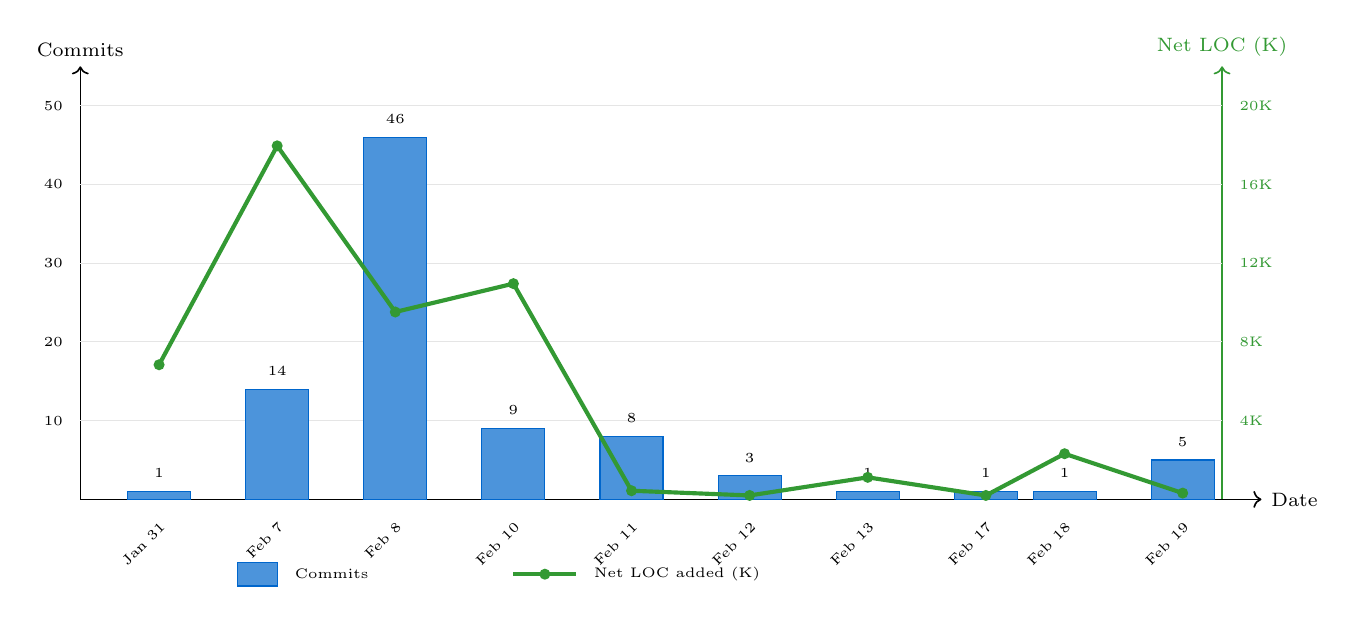
\begin{tikzpicture}[
  bar/.style={fill=extblue!70, draw=extblue, line width=0.4pt},
  addbar/.style={fill=webgreen!60, draw=webgreen!80, line width=0.4pt},
]
  % Constants
  \def\W{14.5}  % chart width

  % Axes
  \draw[->, line width=0.6pt] (0,0) -- (\W+0.5,0) node[right, font=\scriptsize] {Date};
  \draw[->, line width=0.6pt] (0,0) -- (0,5.5) node[above, font=\scriptsize] {Commits};

  % Second y-axis (right) for LOC
  \draw[->, line width=0.6pt, webgreen!80] (\W,0) -- (\W,5.5) node[above, font=\scriptsize, webgreen!80] {Net LOC (K)};

  % Grid lines
  \foreach \y in {1,2,3,4,5} {
    \draw[gray!20, line width=0.3pt] (0,\y) -- (\W,\y);
  }

  % Y-axis ticks (left: commits)
  \foreach \y/\lab in {1/10, 2/20, 3/30, 4/40, 5/50} {
    \node[font=\tiny, anchor=east] at (-0.1, \y) {\lab};
  }

  % Y-axis ticks (right: net LOC in thousands)
  \foreach \y/\lab in {1/4, 2/8, 3/12, 4/16, 5/20} {
    \node[font=\tiny, anchor=west, webgreen!80] at (\W+0.1, \y) {\lab K};
  }

  % Bar positions: 10 bars at x = 1, 2.5, 4, 5.5, 7, 8.5, 10, 11.5, 12.5, 14.0
  % Bar half-width = 0.4

  % Jan 31: 1 commit (0.1)
  \draw[bar] (0.6,0) rectangle (1.4, 0.1);
  \node[font=\tiny, anchor=south] at (1.0, 0.15) {1};

  % Feb 7: 14 commits (1.4)
  \draw[bar] (2.1,0) rectangle (2.9, 1.4);
  \node[font=\tiny, anchor=south] at (2.5, 1.45) {14};

  % Feb 8: 46 commits (4.6)
  \draw[bar] (3.6,0) rectangle (4.4, 4.6);
  \node[font=\tiny, anchor=south] at (4.0, 4.65) {46};

  % Feb 10: 9 commits (0.9)
  \draw[bar] (5.1,0) rectangle (5.9, 0.9);
  \node[font=\tiny, anchor=south] at (5.5, 0.95) {9};

  % Feb 11: 8 commits (0.8)
  \draw[bar] (6.6,0) rectangle (7.4, 0.8);
  \node[font=\tiny, anchor=south] at (7.0, 0.85) {8};

  % Feb 12: 3 commits (0.3)
  \draw[bar] (8.1,0) rectangle (8.9, 0.3);
  \node[font=\tiny, anchor=south] at (8.5, 0.35) {3};

  % Feb 13: 1 commit (0.1)
  \draw[bar] (9.6,0) rectangle (10.4, 0.1);
  \node[font=\tiny, anchor=south] at (10.0, 0.15) {1};

  % Feb 17: 1 commit (0.1)
  \draw[bar] (11.1,0) rectangle (11.9, 0.1);
  \node[font=\tiny, anchor=south] at (11.5, 0.15) {1};

  % Feb 18: 1 commit (0.1)
  \draw[bar] (12.1,0) rectangle (12.9, 0.1);
  \node[font=\tiny, anchor=south] at (12.5, 0.15) {1};

  % Feb 19: 5 commits (0.5)
  \draw[bar] (13.6,0) rectangle (14.4, 0.5);
  \node[font=\tiny, anchor=south] at (14.0, 0.55) {5};

  % Net LOC line (net additions scaled: /4000)
  % Jan 31: 6848  = 1.71
  % Feb 7:  17973 = 4.49
  % Feb 8:  9503  = 2.38
  % Feb 10: 10974 = 2.74
  % Feb 11: 458   = 0.11
  % Feb 12: 17    = 0.05 (clamped)
  % Feb 13: 1112  = 0.28
  % Feb 17: 0     = 0.05 (clamped)
  % Feb 18: 2320  = 0.58
  % Feb 19: 307   = 0.08
  \draw[addbar, line width=1.5pt, fill=none, draw=webgreen!80]
    (1.0, 1.71) -- (2.5, 4.49) -- (4.0, 2.38) -- (5.5, 2.74) -- (7.0, 0.11)
    -- (8.5, 0.05) -- (10.0, 0.28) -- (11.5, 0.05) -- (12.5, 0.58) -- (14.0, 0.08);
  \foreach \x/\y in {1.0/1.71, 2.5/4.49, 4.0/2.38, 5.5/2.74, 7.0/0.11,
                      8.5/0.05, 10.0/0.28, 11.5/0.05, 12.5/0.58, 14.0/0.08} {
    \fill[webgreen!80] (\x,\y) circle (2pt);
  }

  % X-axis labels (rotated 45 degrees)
  \node[font=\tiny, rotate=45, anchor=north east] at (1.0, -0.1) {Jan 31};
  \node[font=\tiny, rotate=45, anchor=north east] at (2.5, -0.1) {Feb 7};
  \node[font=\tiny, rotate=45, anchor=north east] at (4.0, -0.1) {Feb 8};
  \node[font=\tiny, rotate=45, anchor=north east] at (5.5, -0.1) {Feb 10};
  \node[font=\tiny, rotate=45, anchor=north east] at (7.0, -0.1) {Feb 11};
  \node[font=\tiny, rotate=45, anchor=north east] at (8.5, -0.1) {Feb 12};
  \node[font=\tiny, rotate=45, anchor=north east] at (10.0, -0.1) {Feb 13};
  \node[font=\tiny, rotate=45, anchor=north east] at (11.5, -0.1) {Feb 17};
  \node[font=\tiny, rotate=45, anchor=north east] at (12.5, -0.1) {Feb 18};
  \node[font=\tiny, rotate=45, anchor=north east] at (14.0, -0.1) {Feb 19};

  % Legend
  \draw[bar] (2.0, -1.1) rectangle (2.5, -0.8);
  \node[font=\tiny, anchor=west] at (2.6, -0.95) {Commits};
  \draw[webgreen!80, line width=1.5pt] (5.5, -0.95) -- (6.3, -0.95);
  \fill[webgreen!80] (5.9, -0.95) circle (2pt);
  \node[font=\tiny, anchor=west] at (6.4, -0.95) {Net LOC added (K)};

\end{tikzpicture}
\caption{Daily commit activity (blue bars, left axis) and net lines of code added (green line, right axis) across the ten active development days. February~8 was the most intensive session with 46~commits, while February~7 produced the highest net code additions (+18K~lines) as the web platform and extension foundations were built simultaneously. The later days (Feb~12--18) reflect documentation, paper preparation, and refinement work with lower churn. February~19 added VS~Code~1.109 agent-skills and hooks documentation, wiki scheduling, and events-page fixes (5~commits, +307~LOC net).}
\label{fig:commits}
\end{figure*}



\subsection{Codebase composition}

Table~\ref{tab:codebase} breaks down the current codebase by component.

\begin{table}[htp!]
\centering
\small
\begin{tabular}{|l|r|r|}
\hline
\textbf{Component} & \textbf{LOC} & \textbf{Files} \\
\hline
VS~Code Extension (source) & 4,986 & 12 \\
\hline
Extension tests & 2,663 & 10 \\
\hline
MCP Server + CLI (\texttt{tokalator-mcp/}) & 650 & 8 \\
\hline
Web platform library (\texttt{lib/}) & 3,243 & 10 \\
\hline
Library tests & 899 & 4 \\
\hline
React components & 4,811 & 22 \\
\hline
App pages (\texttt{app/}) & 3,675 & 28 \\
\hline
Content (JSON) & 1,795 & 5 \\
\hline
\textbf{Total TypeScript/TSX} & \textbf{20,814} & -- \\
\hline
\end{tabular}
\caption{Codebase composition by component (v3.1.1). Test code represents 17.1\% of the total codebase (3,562 out of 20,814 LOC), indicating substantial testing investment. The MCP Server + CLI (\texttt{tokalator-mcp/}) adds $\sim$650 LOC across 8 source files.}
\label{tab:codebase}
\end{table}

\subsection{Test distribution}

Figure~\ref{fig:testdist} visualizes the distribution of the 124 test cases across the 6 test files.

\begin{figure*}[htp!]
\centering
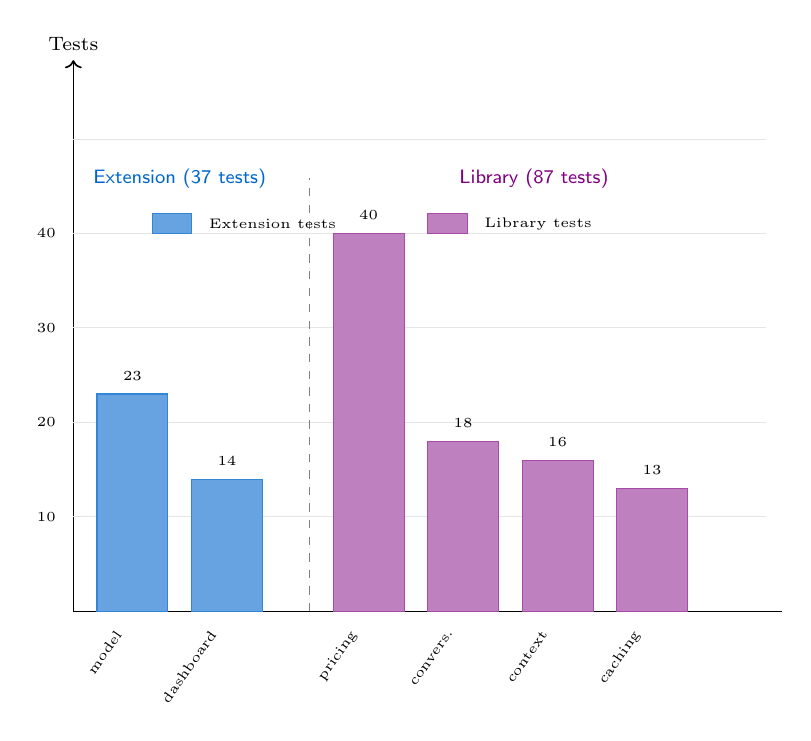
\begin{tikzpicture}[
  extbar/.style={fill=extblue!60, draw=extblue!80, line width=0.4pt},
  libbar/.style={fill=catpurple!50, draw=catpurple!70, line width=0.4pt},
]
  % Axes
  \draw[->, line width=0.6pt] (0,0) -- (0,7.0) node[above, font=\scriptsize] {Tests};
  \draw[line width=0.6pt] (0,0) -- (9.0,0);

  % Grid lines
  \foreach \y in {1,...,5} {
    \draw[gray!20, line width=0.3pt] (0,\y*1.2) -- (8.8,\y*1.2);
  }

  % Y-axis ticks (scaled: value * 0.15)
  \foreach \y/\lab in {1.2/10, 2.4/20, 3.6/30, 4.8/40} {
    \node[font=\tiny, anchor=east] at (-0.1, \y) {\lab};
  }

  % Extension test bars (2 files)
  \draw[extbar] (0.3,0) rectangle (1.2, 2.76);   % modelProfiles: 23
  \node[font=\tiny, anchor=south] at (0.75, 2.81) {23};

  \draw[extbar] (1.5,0) rectangle (2.4, 1.68);   % dashboardProvider: 14
  \node[font=\tiny, anchor=south] at (1.95, 1.73) {14};

  % Separator line
  \draw[gray, dashed, line width=0.4pt] (3.0, 0) -- (3.0, 5.5);

  % Library test bars (4 files)
  \draw[libbar] (3.3,0) rectangle (4.2, 4.8);   % pricing: 40
  \node[font=\tiny, anchor=south] at (3.75, 4.85) {40};

  \draw[libbar] (4.5,0) rectangle (5.4, 2.16);   % conversation: 18
  \node[font=\tiny, anchor=south] at (4.95, 2.21) {18};

  \draw[libbar] (5.7,0) rectangle (6.6, 1.92);   % context: 16
  \node[font=\tiny, anchor=south] at (6.15, 1.97) {16};

  \draw[libbar] (6.9,0) rectangle (7.8, 1.56);   % caching: 13
  \node[font=\tiny, anchor=south] at (7.35, 1.61) {13};

  % X-axis labels (rotated)
  \foreach \x/\lab in {
    0.75/{\rotatebox{55}{\tiny model}},
    1.95/{\rotatebox{55}{\tiny dashboard}},
    3.75/{\rotatebox{55}{\tiny pricing}},
    4.95/{\rotatebox{55}{\tiny convers.}},
    6.15/{\rotatebox{55}{\tiny context}},
    7.35/{\rotatebox{55}{\tiny caching}}
  } {
    \node[anchor=north east] at (\x, -0.1) {\lab};
  }

  % Labels
  \node[font=\scriptsize\sffamily, extblue] at (1.35, 5.5) {Extension (37 tests)};
  \node[font=\scriptsize\sffamily, catpurple] at (5.85, 5.5) {Library (87 tests)};

  % Legend
  \draw[extbar] (1.0, 4.8) rectangle (1.5, 5.05);
  \node[font=\tiny, anchor=west] at (1.6, 4.925) {Extension tests};
  \draw[libbar] (4.5, 4.8) rectangle (5.0, 5.05);
  \node[font=\tiny, anchor=west] at (5.1, 4.925) {Library tests};

\end{tikzpicture}
\caption{Distribution of 124 test cases across 6 test files. Extension tests (blue, left of dashed line) cover 2 modules; library tests (purple, right) cover 4 shared modules. The most-tested module is the Pricing Engine (40 tests), reflecting its critical role in cost calculations across all 15 models.}
\label{fig:testdist}
\end{figure*}


\subsection{AI-assisted development sessions}


All sessions used GitHub Copilot (VS~Code) for inline code completion and Claude (Anthropic) for interactive pair-programming via chat. The AI tools accelerated implementation; all design decisions, architectural choices, and mathematical formulations were made by the authors. The cumulative Git statistics across all 89 commits are: \textit{+67,834} insertions and \textit{--18,228} deletions, yielding a net codebase of $\sim$50K lines (including content, configuration, and documentation). The current TypeScript/TSX codebase totals \textit{20,814~LOC} (Table~\ref{tab:codebase}), indicating that approximately 69\% of all code written was later refactored or replaced, a natural consequence of the iterative, AI-assisted development workflow where rapid prototyping is followed by manual refinement.




\printcredits

\bibliographystyle{cas-model2-names}

% Loading bibliography database
\bibliography{references}

\end{document}

